\chapter{Cyclic Coordinate Descent}
For the implementation of the da Vinci Surgical System in the operating theatre simulation a Cyclic Coordinate Descent (CCD) inverse kinematic (IK) method is used. The IK finds values for all connected joints so that an end-effector reaches a desired position and orientation. Chin et al compares different solutions to the IK proble \citep{kwan_wu_chin_closed-form_1997}. CCD is an optimisation method for minimising a nonlinear cost function. The method iterates through a list of variables and adjusts the values to minimise the cost. The use of CCD to solve the IK problem is documented by Wang and Chen \citep{wang_combined_1991-1}. CCD iterates through all joints one at a time starting from the outermost one. For each joint an angle is chosen which moves the end-effector closest to the desired position.
\begin{figure}[h]
\centering
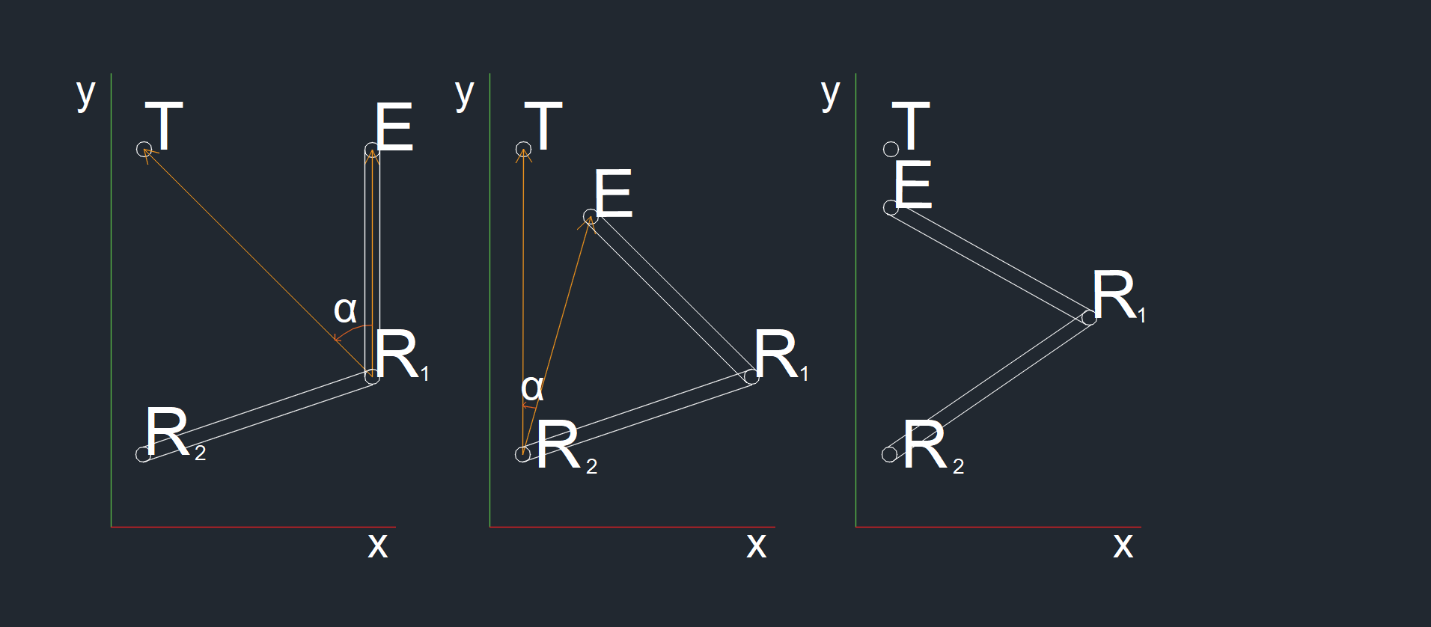
\includegraphics[width=\textwidth]{CCD/IKCCD.png}
\caption{Visual example of IK using CCD }
\label{fig:figifig}
\end{figure}

In \autoref{fig:figifig}, a desired position T, end-effector position E and position of the current joint R1 is shown. Calculating the rotation for R1 is achieved by calculating the dot product R1 $\overline{R_1T} \cdot \overline{R_1E}$  and the cross product $R1_T \times R1_E$, in both cases the vectors should be normalised. Using inverse cosine of the dot product, it is possible to get the angle between the two vectors, and the cross product is used to show the direction in which the root (In this case $R_1$) needs to be rotated. In 2D the sign of the cross product is used, however in 3D the normalised cross product vector is multiplied by the angle between the two vectors providing three new angles, for each of the three axes respectively. Those angles are directly added to the current rotation of the root joint. This process is repeated for each joint in the list.

One addition to the algorithm is the implementation of a restriction vector. The restriction is a unit vector (for example [0,0,1]), when multiplied by the new rotation vector it effectively removes any rotation from two of the axes, allowing rotation to happen only around one. This allows for more realistic movement by not allowing joints to rotate in unnatural ways.
 \begin{figure}[h]
 \centering
 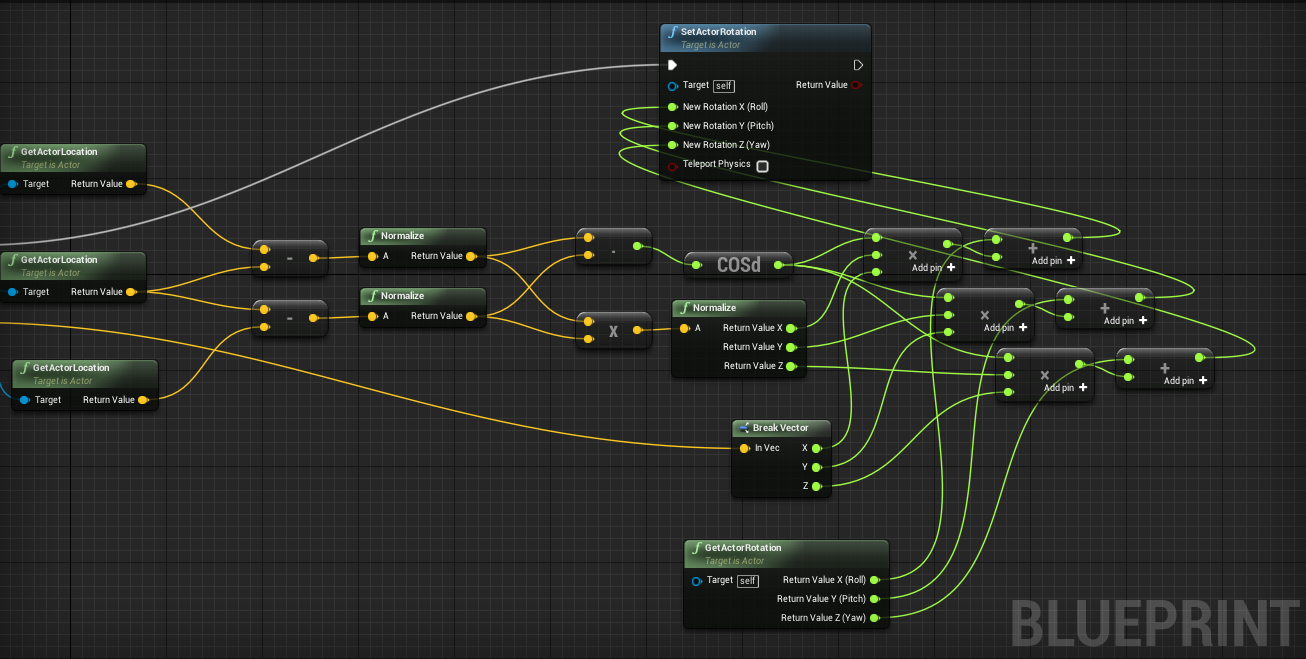
\includegraphics[width=\textwidth]{CCD/CCDBlueprint.png}
 \caption{Blueprint that changes the rotation of an object to position the end-effector closest to the desired target}
 \label{fig:blueprint}
 \end{figure}
 
\autoref{fig:blueprint} shows the implementation in Unreal Engine.
Because Unreal Engine does not allow for easy manipulation of dedicated bone structures in real time a hierarchical joint system was used instead. Each joint shares a parent-child relationship with other joints in the chain, and any changes made to the transform of a parent joint affects all of its children.

